
\begin{frame}{[\textbf{Chapter 5}] 結合関数推定}

\begin{figure}
  \centering
  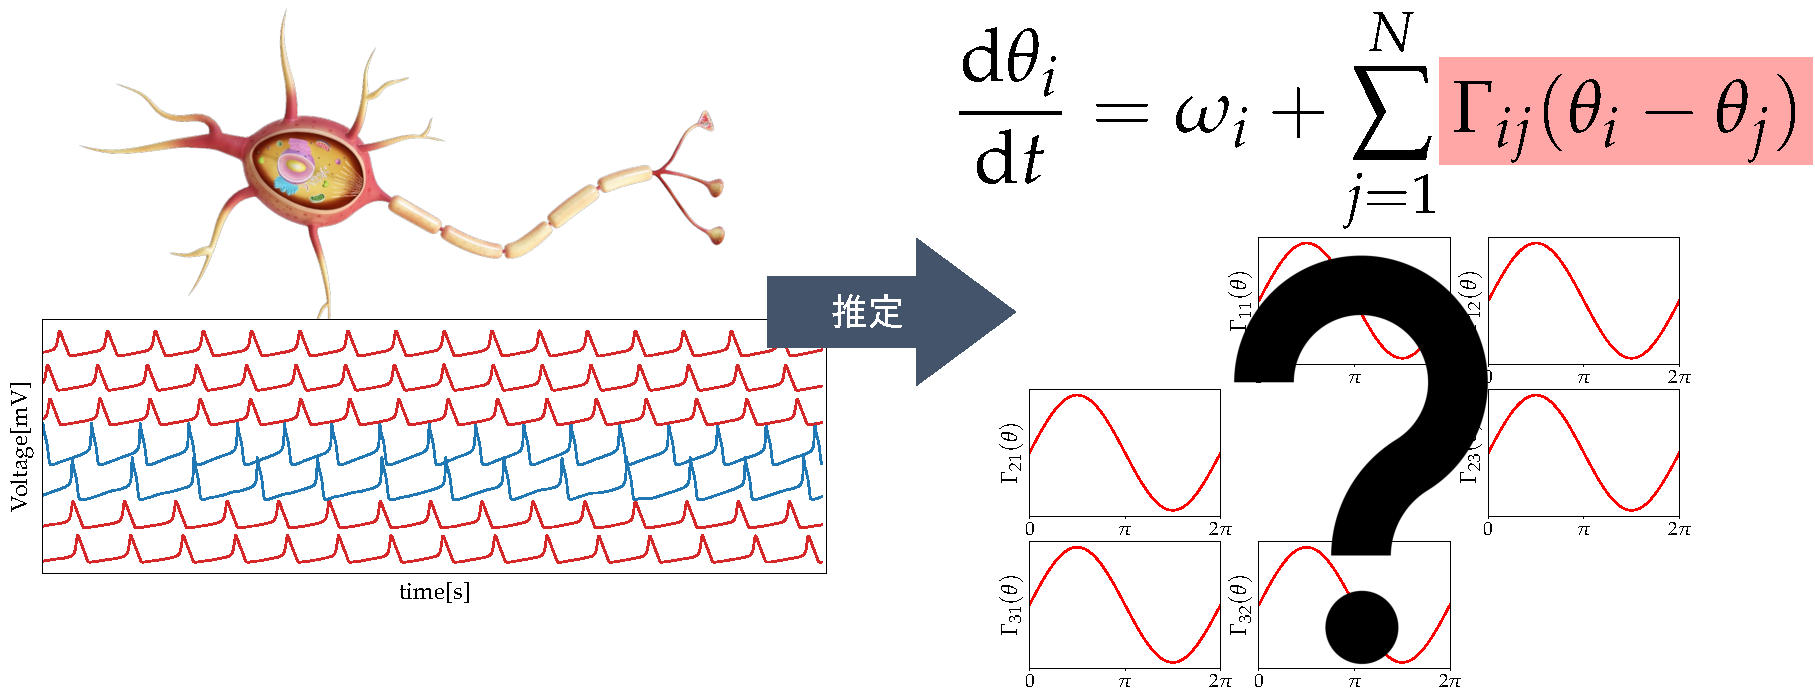
\includegraphics[width=\textwidth]{figs/gp_coupling_ponchi.pdf}
\end{figure}

\begin{itemize}
  \item 先行研究: \textbf{ベイズ線形回帰} [Ota 2018]
  \begin{itemize}
    \item $\Gamma_{ij}$を有限次のFourier級数展開で近似し、Fourier係数を線形回帰
    \item 何次まで展開すべきかの自由度が残る
    \item Gibbs現象が生じる場合も
  \end{itemize}
  \item 本研究: \underline{\textbf{ガウス過程回帰を用いて結合関数を推定できるか?}}
  \begin{itemize}
    \item ``滑らかな周期関数''なる関数空間の中で回帰が可能になる
  \end{itemize}
\end{itemize}

\end{frame}

\begin{frame}{ガウス過程}
  \begin{block}{ガウス過程}
    確率過程$X_{t}$について、任意の組$(X_{t_{1}},\dots,X_{t_{k}})$が多次元正規分布に従うとき$X_{t}$を\textbf{ガウス過程}と呼ぶ
  \end{block}
  \begin{align*}
    f\sim\mathcal{GP}(m,k)
  \end{align*}
  \begin{itemize}
    \item $m(x)$: 平均関数
    \item $k(x,\tilde{x})$: カーネル関数
  \end{itemize}
  \begin{figure}
    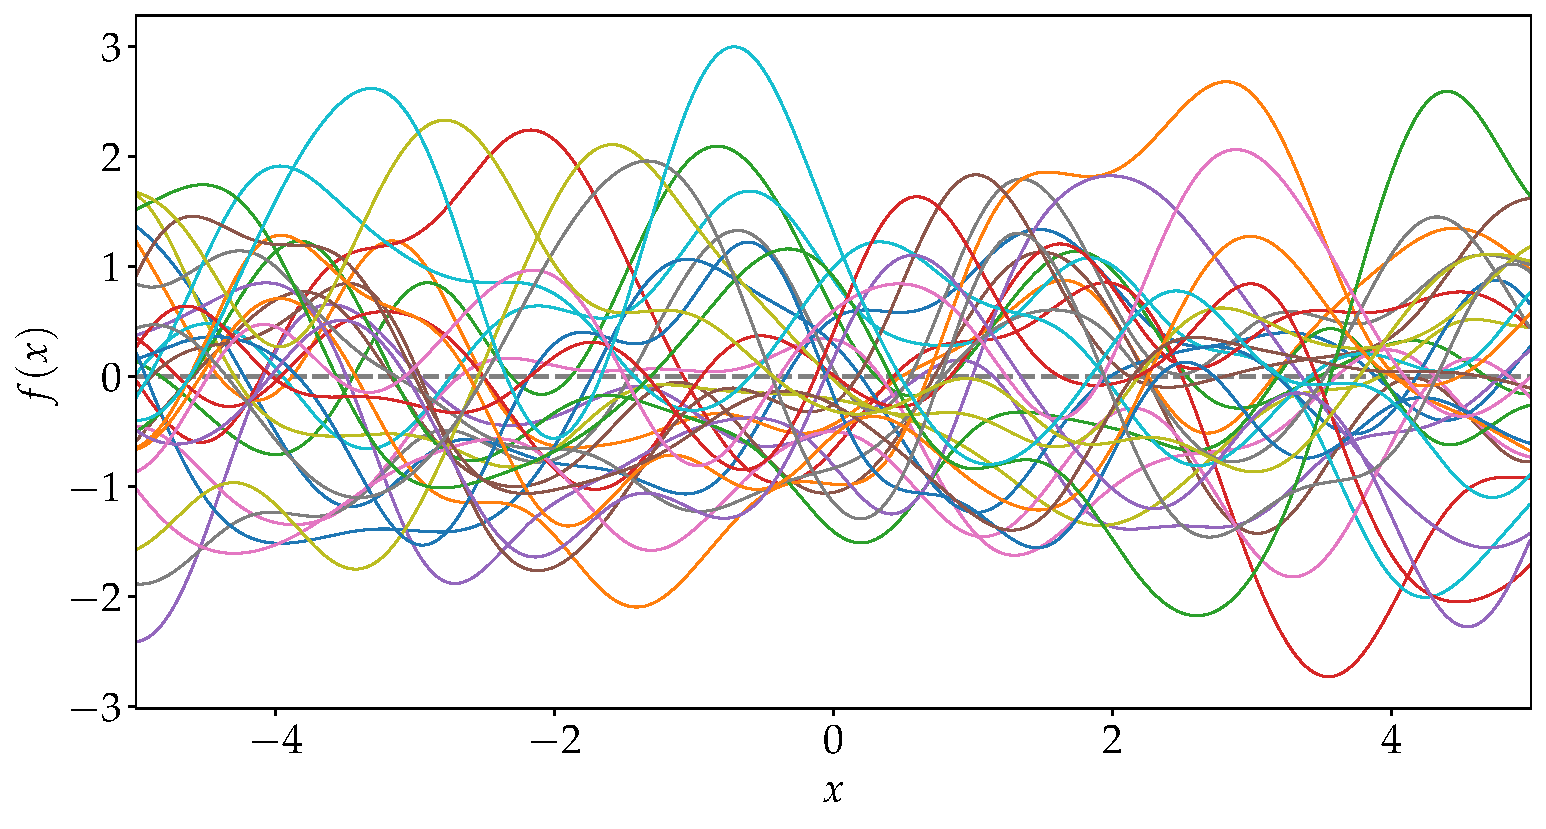
\includegraphics[height=0.4\textheight]{figs/rbf_sample.pdf}
  \end{figure}
\end{frame}

\begin{frame}{カーネル関数}
ガウス過程で生成される関数の性質を決定(e.g. \textbf{滑らかさ}、\textbf{周期性}、\textbf{加法性})
\begin{figure}
  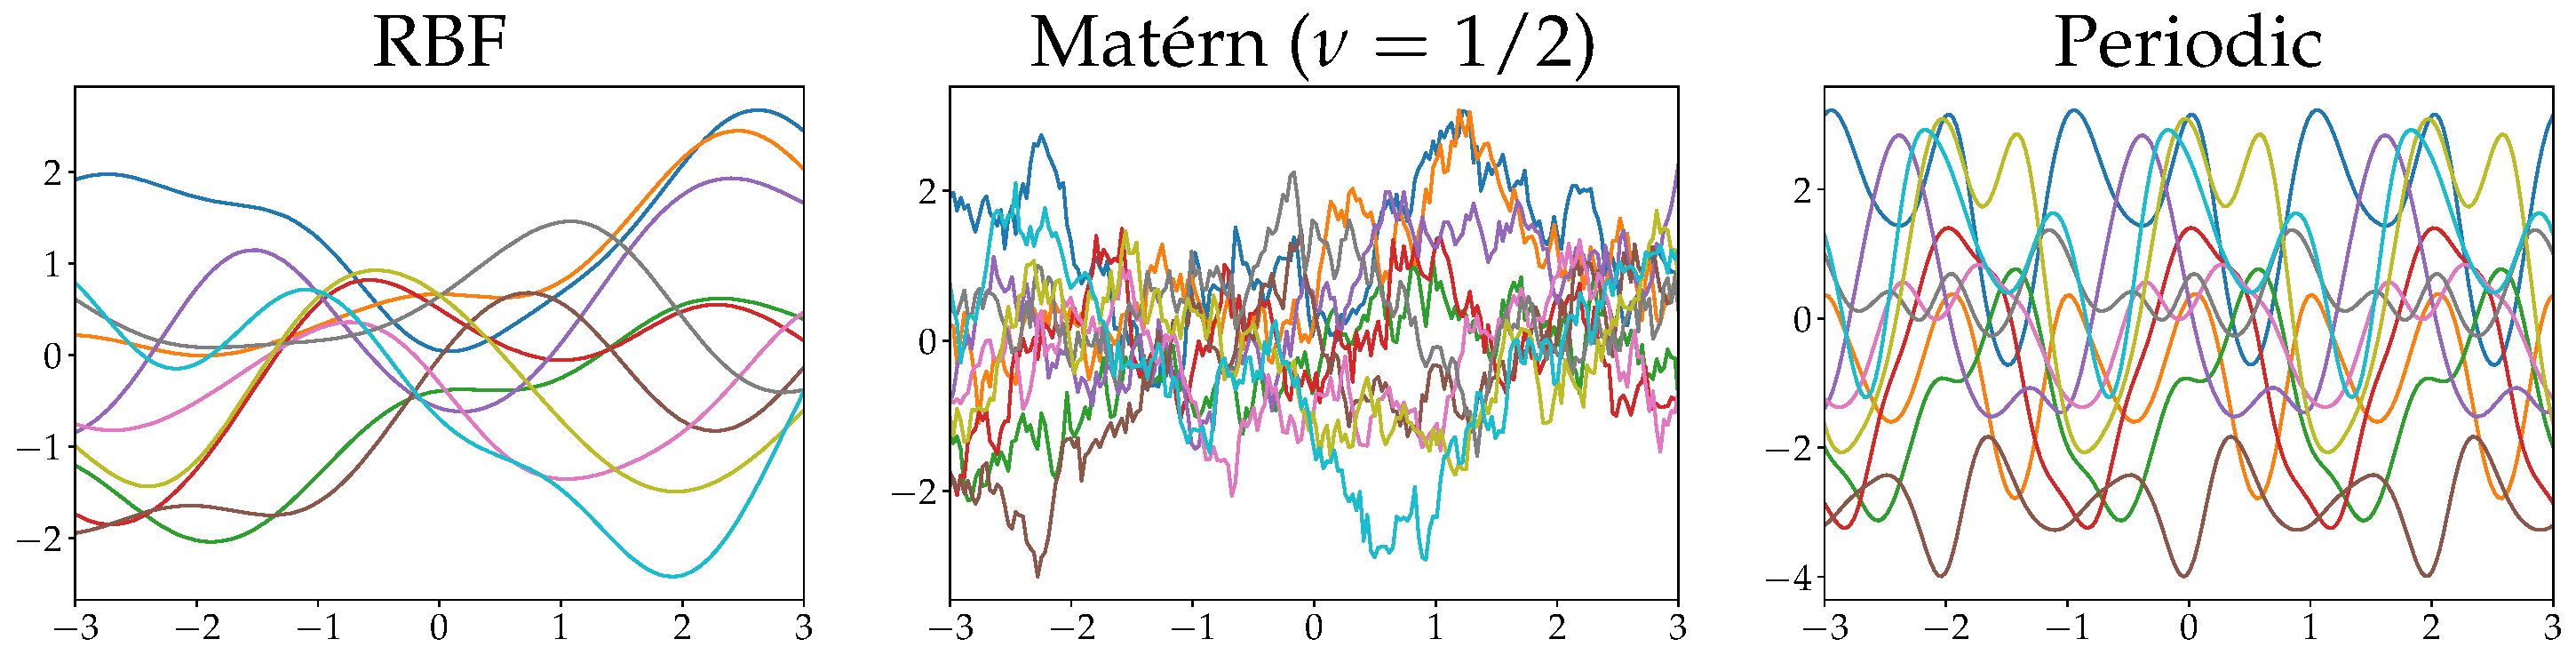
\includegraphics[width=0.6\textwidth]{figs/kernel_comparison.pdf}
\end{figure}
\begin{itemize}
  \item \textbf{additive model} $f(\bm{x})=\sum_{i}f_{i}(x_{i})$
  \begin{itemize}
    \item additiveなカーネルで生成 $k(\bm{x},\bm{\tilde{x}})=\sum_{i}k_{i}(x_{i},\tilde{x}_{i})$
  \end{itemize}
\end{itemize}
\begin{figure}
  \centering
  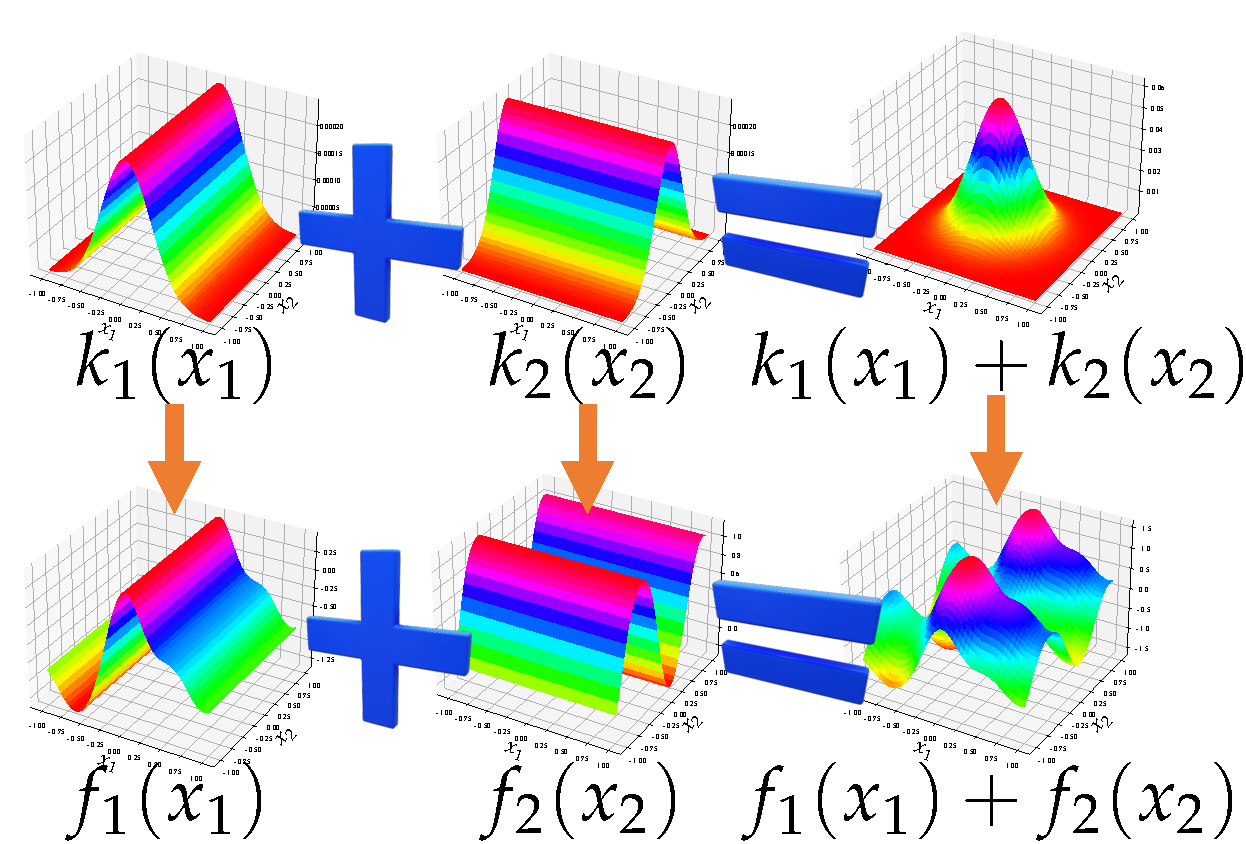
\includegraphics[width=0.5\textwidth]{figs/additive_gp.pdf}
\end{figure}
\end{frame}

\begin{frame}{ガウス過程回帰}
$y=f(x)$を満たすデータ$\mathcal{D}=\{(x_{i},y_{i})\}_{i}$によるガウス過程の事後分布で回帰\footnote{$[k_{XX}]_{ij}=k(x_{i},x_{j}),[k_{xX}]_{i}=k(x_{i},x),[\bm{y}]_{i}=y_{i},[m_{X}]_{i}=m(x_{i})$}
\begin{align*}
  &f\mid\mathcal{D}\sim\mathcal{GP}(\overline{m},\overline{k}),\\
  &\overline{m}(x)=m(x)+k_{xX}{k_{XX}}^{-1}(\bm{y}-m_{X}),\\
  &\overline{k}(x,\tilde{x})=k(x,\tilde{x})-k_{xX}{k_{XX}}^{-1}k_{X\tilde{x}}
\end{align*}
\begin{itemize}
  \item[\checkmark] \underline{ガウス過程のデータによる事後分布はまたガウス過程}
  \item[\checkmark] ハイパーパラメータは対数尤度最大化で最適化
  % \item[\checkmark] データ数$n$に対して$\mathcal{O}(n^{3})$の計算量が必要 $\Longrightarrow$ SVGPによる効率化
\end{itemize}
\begin{figure}
  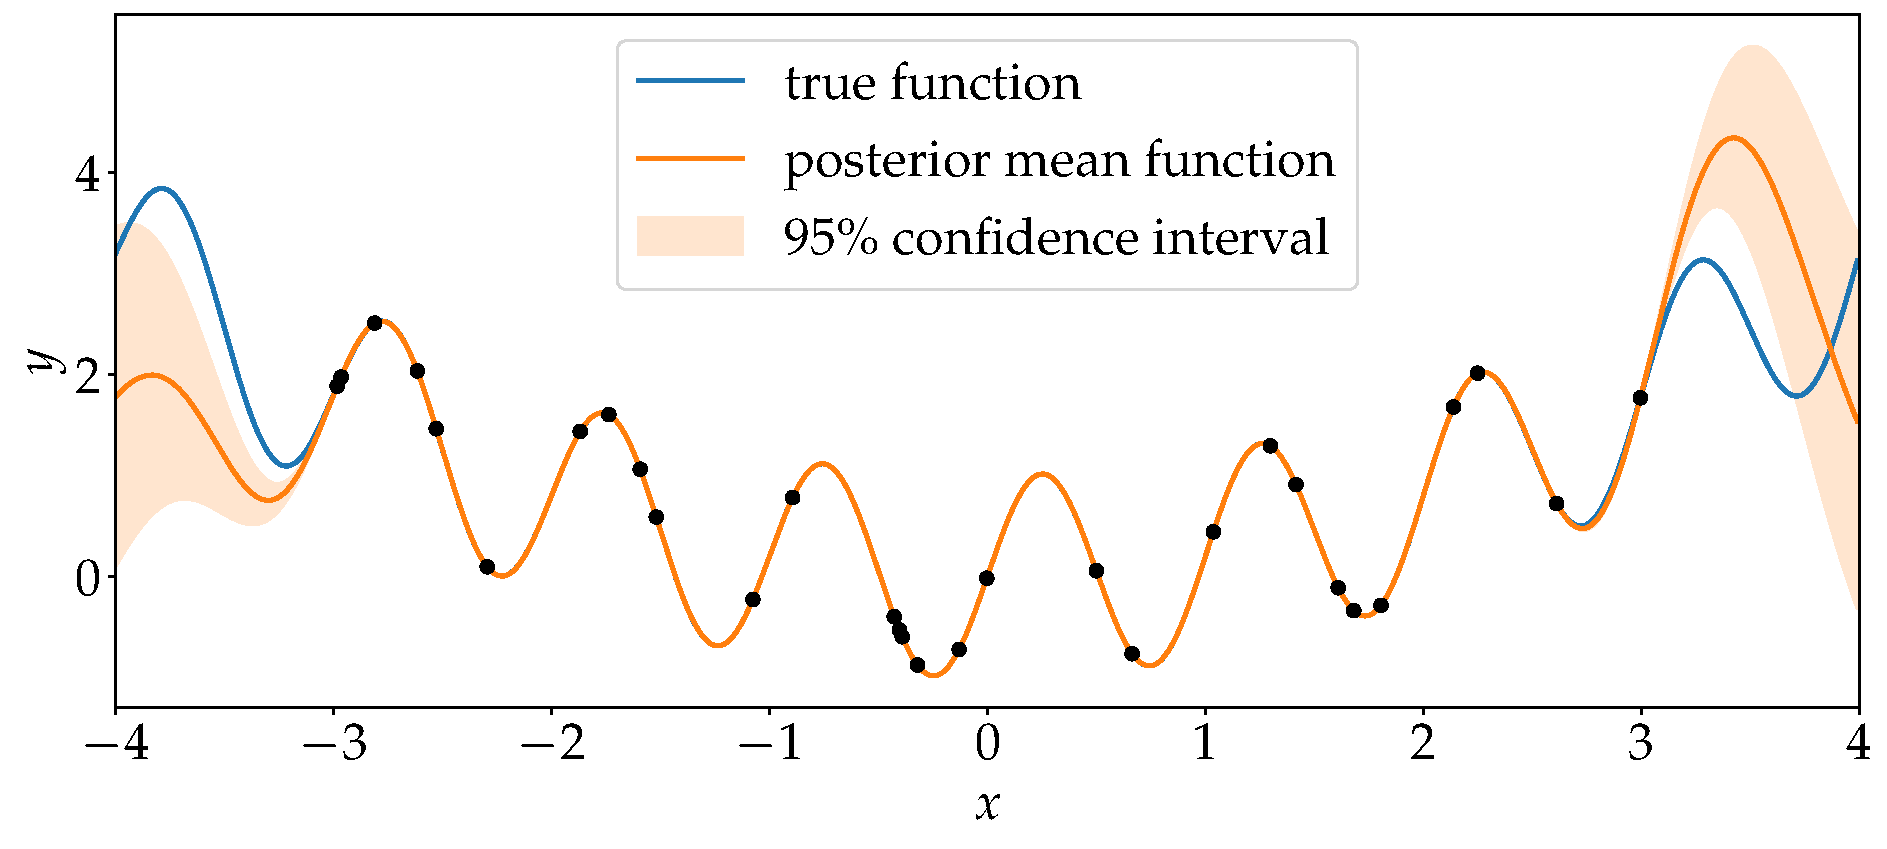
\includegraphics[height=0.35\textheight]{figs/gpr_sample.pdf}
\end{figure}
\end{frame}

\begin{frame}{大規模データに対する処方箋}

  \begin{itemize}
    \item[\checkmark] データ数$n$に対して$\mathcal{O}(n^{3})$の計算量\\
    $\Longrightarrow$ 大規模データに対しては効率的な計算が必要
    \item \textbf{補助変数法(sparse GP)} [Quiñonero-Candela 2005]
    \begin{itemize}
      \item $m(<n)$個の補助入力点を用いて計算を効率化
    \end{itemize}
    \item \textbf{変分ベイズ法(SVGP)} [Hensman 2013]
    \begin{itemize}
      \item $m(<n)$個の補助入力点を用意
      \item 変分事後分布を学習し真の事後分布に近似
      \item データをサイズ$b$のミニバッチにわけることで学習を効率化
    \end{itemize}
  \end{itemize}
  
  \begin{table}[H]
    \caption*{計算量の比較}
    \begin{tabular}{l|cc>{\columncolor[rgb]{1.0,1.0,0.7}}c}
      & GP & sparse GP & SVGP \\\hline\hline
     推論コスト & $\mathcal{O}(n^{3})$ & $\mathcal{O}(nm^{2})$ & $\mathcal{O}(bm^{2}+m^{3})$ \\
     メモリコスト & $\mathcal{O}(n^{2})$ & $\mathcal{O}(nm)$ & $\mathcal{O}(bm+m^{2})$ \\
    \end{tabular}
  \end{table}
  
  \begin{itemize}
    \item 本研究ではSVGPを用いる
  \end{itemize}
\end{frame}

% \begin{frame}{アルゴリズム}
% \begin{columns}[t]
%   \begin{column}{0.4\textwidth}
%     \begin{enumerate}
%       \item 時系列の観測 ($N$体)
%       \item 位相への変換
%       \item $i$体目のベクトル場について
%       \begin{enumerate}
%         \item ベクトル場のデータ$\mathcal{D}_{i}$を生成
%         \begin{align*}
%           \mathcal{D}_{i}=\{(\bm{x}_{k},y_{k})\}_{k=1}^{n}
%         \end{align*}
%         \item SVGPで結合関数を推定
%       \end{enumerate}
%     \end{enumerate}
%   \end{column}
%   \begin{column}{0.6\textwidth}
%     \begin{itemize}
%       \item 時系列データの位相への変換
%       \begin{itemize}
%         \item 偏角もしくはヒルベルト変換
%         \item Kralemannの方法\footnote{Kralemann 2007}
%       \end{itemize}
%       \item ガウス過程回帰に用いるカーネル関数
%       \begin{align*}
%         k(\bm{x},\tilde{\bm{x}})=\sum_{j=1}^{N-1}\theta_{0}^{(j)}\exp(\theta_{1}^{(j)}\cos(x_{j}-\tilde{x}_{j}))
%       \end{align*}
%       \begin{itemize}
%         \item $N-1$変数のadditive modelへ回帰
%         \begin{align*}
%           \mathrm{input}:&\  \{\red{\theta_{j}-\theta_{i}}\}_{j\ne i}\\
%           \mathrm{output}:&\  \omega_{i}+\sum_{j\ne i}\Gamma_{ij}(\red{\theta_{j}-\theta_{i}})\\
%           \mathrm{target}:&\ \frac{\diff\theta_{i}}{\diff t}\simeq\frac{\theta_{i}(t_{k+1})-\theta_{i}(t_{k})}{t_{k+1}-t_{k}}
%         \end{align*}
%       \end{itemize}
%     \end{itemize}
%   \end{column}
% \end{columns}
% \end{frame}

\begin{frame}[t]{[提案手法] 観測・位相へ変換}
\begin{figure}
  \centering
  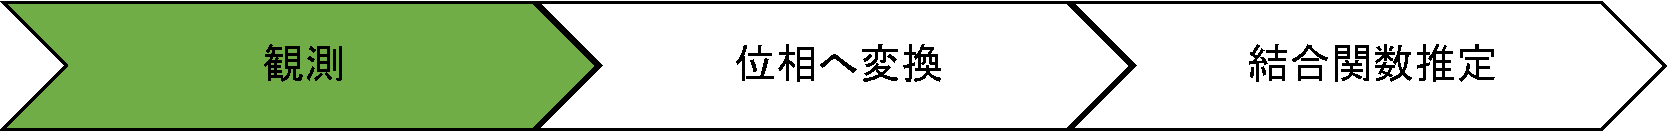
\includegraphics[width=\textwidth]{figs/flowchart1.pdf}
\end{figure}
\begin{figure}
  \centering
  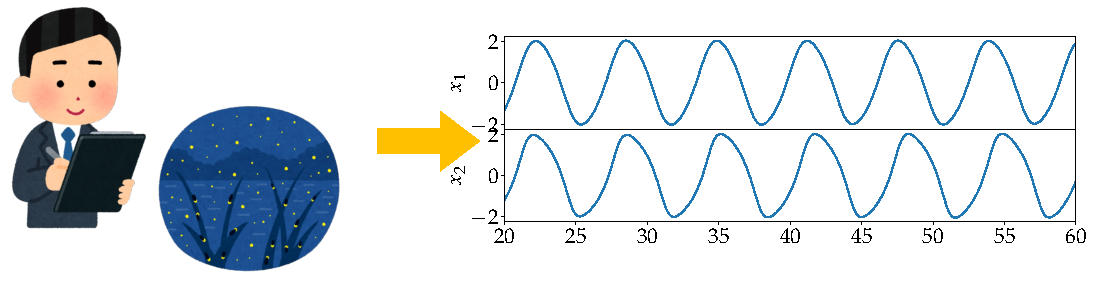
\includegraphics[width=0.7\textwidth]{figs/observe_ponchi.pdf}
\end{figure}
\begin{figure}
  \centering
  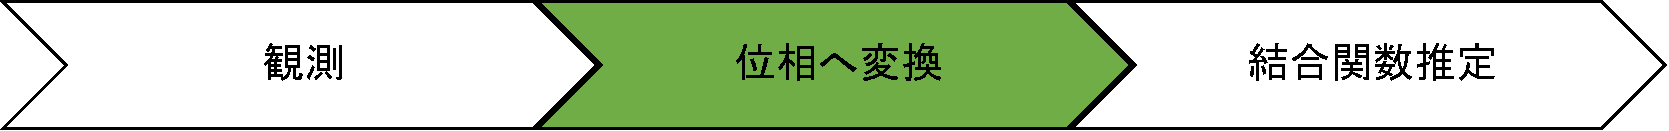
\includegraphics[width=\textwidth]{figs/flowchart2.pdf}
\end{figure}
\begin{itemize}
  \item Kralemannの方法 [Kralemann 2007]
\end{itemize}
\begin{figure}
  \centering
  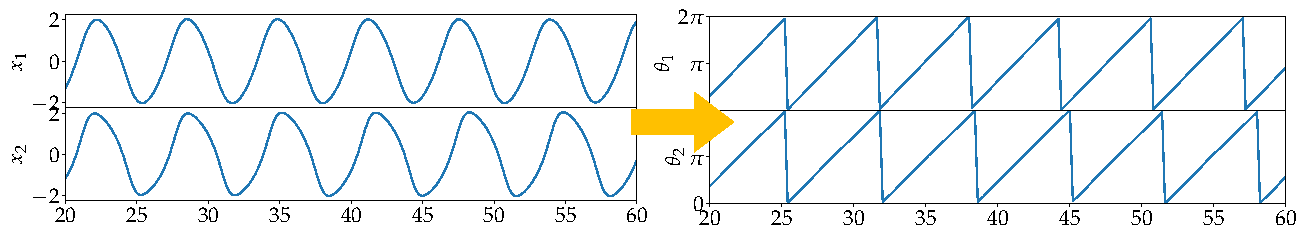
\includegraphics[width=\textwidth]{figs/data_to_phase.pdf}
\end{figure}
\end{frame}


\begin{frame}[t]{[提案手法] 結合関数推定}
  \begin{figure}
    \centering
    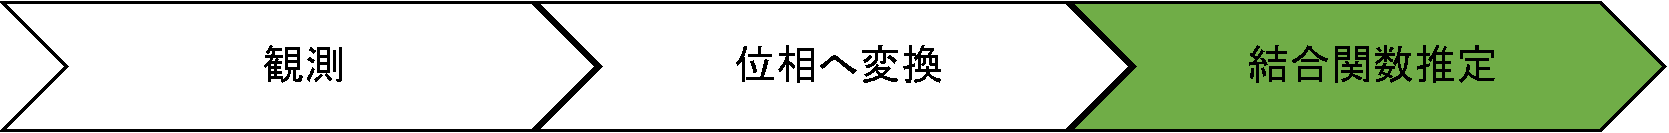
\includegraphics[width=\textwidth]{figs/flowchart3.pdf}
  \end{figure}
  \begin{columns}[t]
    \begin{column}{0.45\textwidth}
      $i$体目のベクトル場について\\
      \checkmark 回帰する関数 $\red{\Gamma_{ij}}\colon\mathbb{S}^{1}\to\mathbb{R}$
      \begin{align*}
        \frac{\diff\theta_{i}}{\diff t}=\sum_{j\ne i}\red{\Gamma_{ij}}(\theta_{j}-\theta_{i})
      \end{align*}
      \checkmark データ$\mathcal{D}_{i}=\{(\bm{x}_{k},y_{k})\}_{k}$
      \begin{align*}
        &\bm{x}_{k}=\begin{bmatrix}
          \theta_{1}(t_{k}) - \theta_{i}(t_{k})\\
          \vdots\\
          \theta_{N}(t_{k}) - \theta_{i}(t_{k})
        \end{bmatrix} \in \mathbb{T}^{N-1}\\
        &y_{k}=\frac{\theta_{i}(t_{k+1}) - \theta_{i}(t_{k})}{t_{k+1} - t_{k}} \in \mathbb{R}
      \end{align*}
    \end{column}
    \begin{column}{0.55\textwidth}
      \checkmark additiveな周期カーネル
      \begin{align*}
        &k(\bm{x},\tilde{\bm{x}})=\sum_{j\ne i}k_{j}(x_{j},\tilde{x}_{j})\\
        &k_{j}(x,\tilde{x})=p_{0}^{(j)}\exp(p_{1}^{(j)}\cos(x-\tilde{x}))
      \end{align*}
      \checkmark SVGPで結合関数を推定
      \begin{align*}
        \red{\Gamma_{ij}\mid\mathcal{D}_{i}}&\sim\mathcal{GP}(\overline{m}_{j}, \overline{k}_{j})\\
        \overline{m}_{j}(x)&=k_{j}(x,X)k(X,X)^{-1}\bm{y}\\
        \overline{k}_{j}(x,\tilde{x})&=k_{j}(x,\tilde{x})\\
        &\quad -k_{j}(x,X)k(X,X)^{-1}k_{j}(X,\tilde{x})
      \end{align*}
    \end{column}
  \end{columns}
\end{frame}

\begin{frame}{van der Pol振動子}
\begin{figure}
  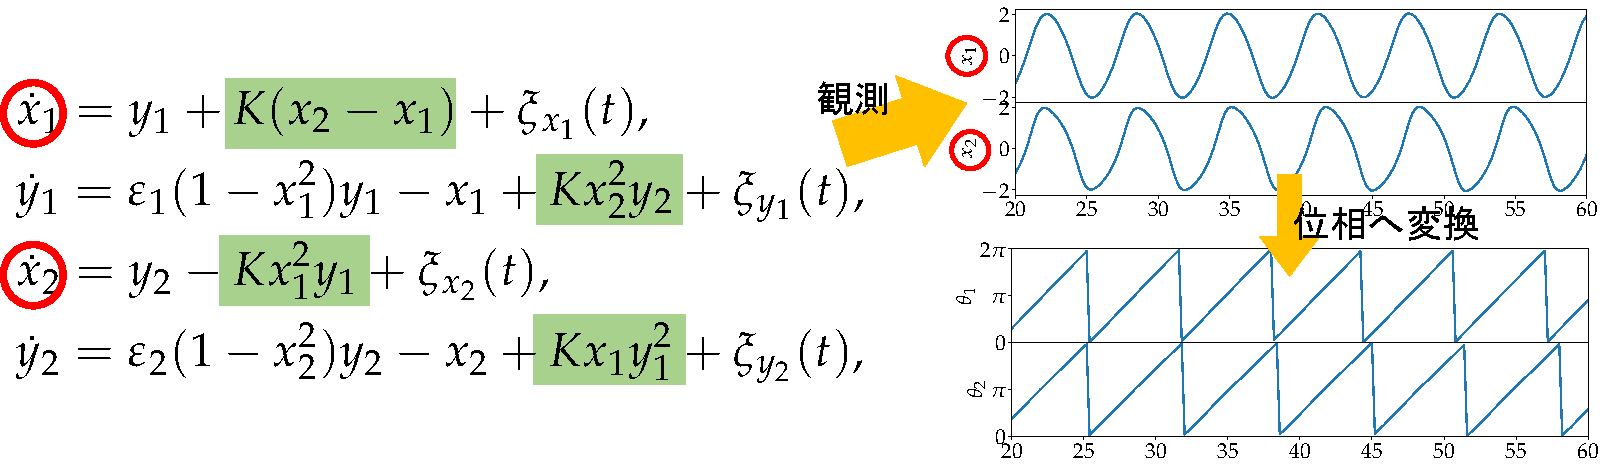
\includegraphics[height=0.35\textheight]{figs/vdp_schematic.pdf}
\end{figure}
\begin{figure}
  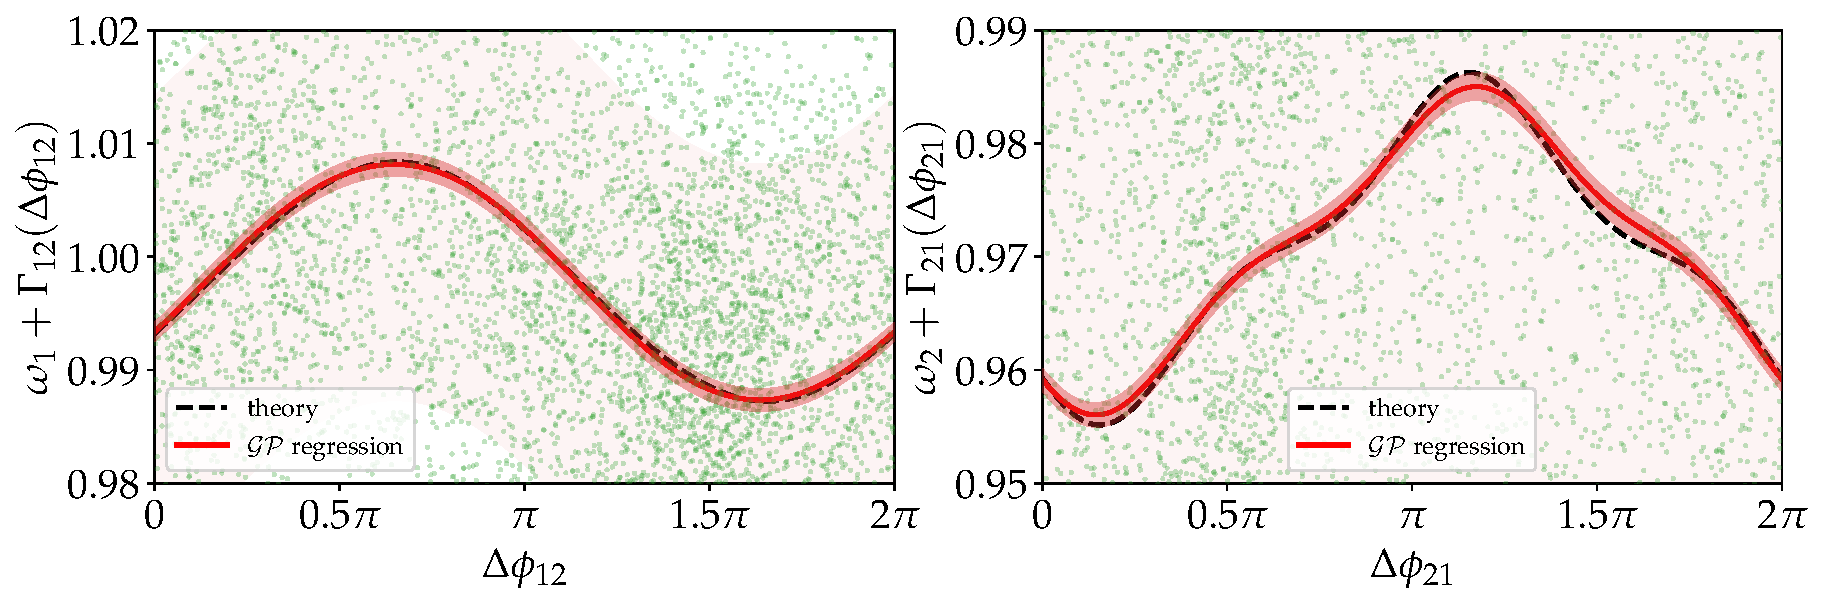
\includegraphics[width=\textwidth]{figs/exp01case01.pdf}
\end{figure}
\end{frame}

\begin{frame}{ベイズ線形回帰との比較}
  \begin{figure}
    \centering
    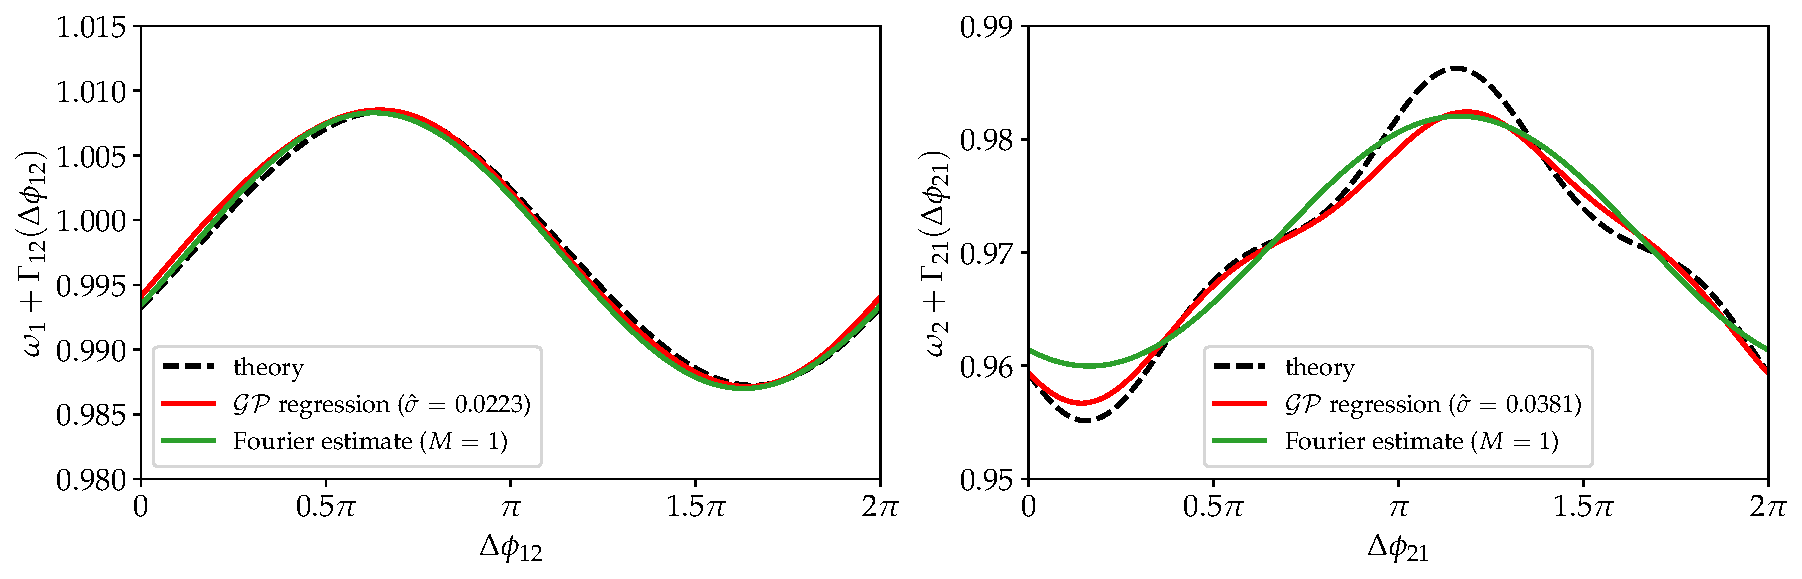
\includegraphics[width=\textwidth]{figs/vdp.pdf}
  \end{figure}
  \begin{itemize}
    \item ベイズ線形回帰はフーリエ級数を何次まで展開するかのモデル選択が必要
    \begin{itemize}
      \item 適切な次数選択に失敗している
    \end{itemize}
    \item ガウス過程回帰は``滑らかな周期関数''なる関数空間全体の中での回帰を行う
  \end{itemize}
\end{frame}

\begin{frame}{神経細胞モデル}
  \begin{columns}[t]
    \begin{column}{0.5\textwidth}
      \checkmark 興奮性・抑制性細胞によるネットワークモデル
      \begin{figure}
        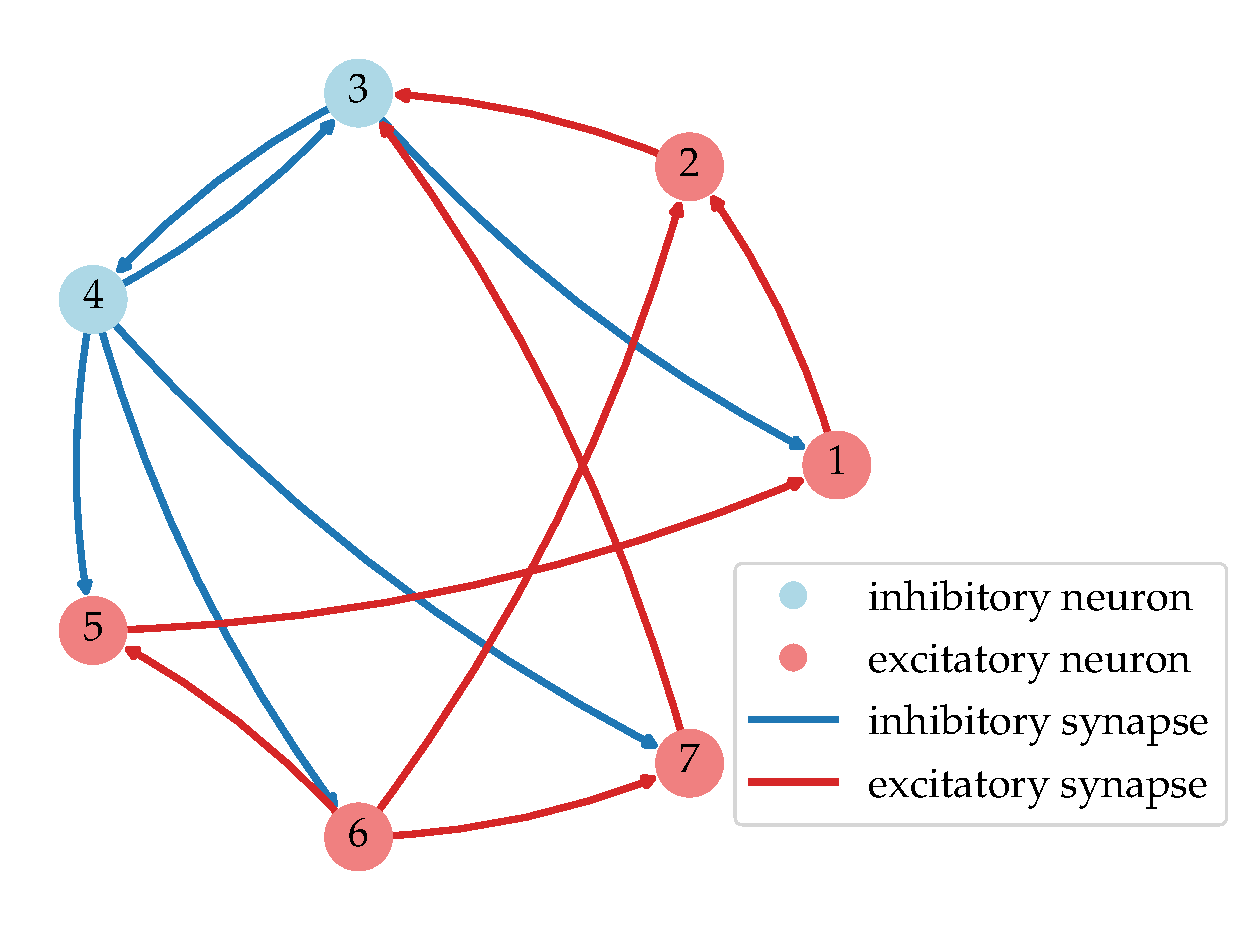
\includegraphics[width=0.9\columnwidth]{figs/snn_netplot.pdf}
      \end{figure}
      \checkmark 観測時系列
      \begin{figure}
        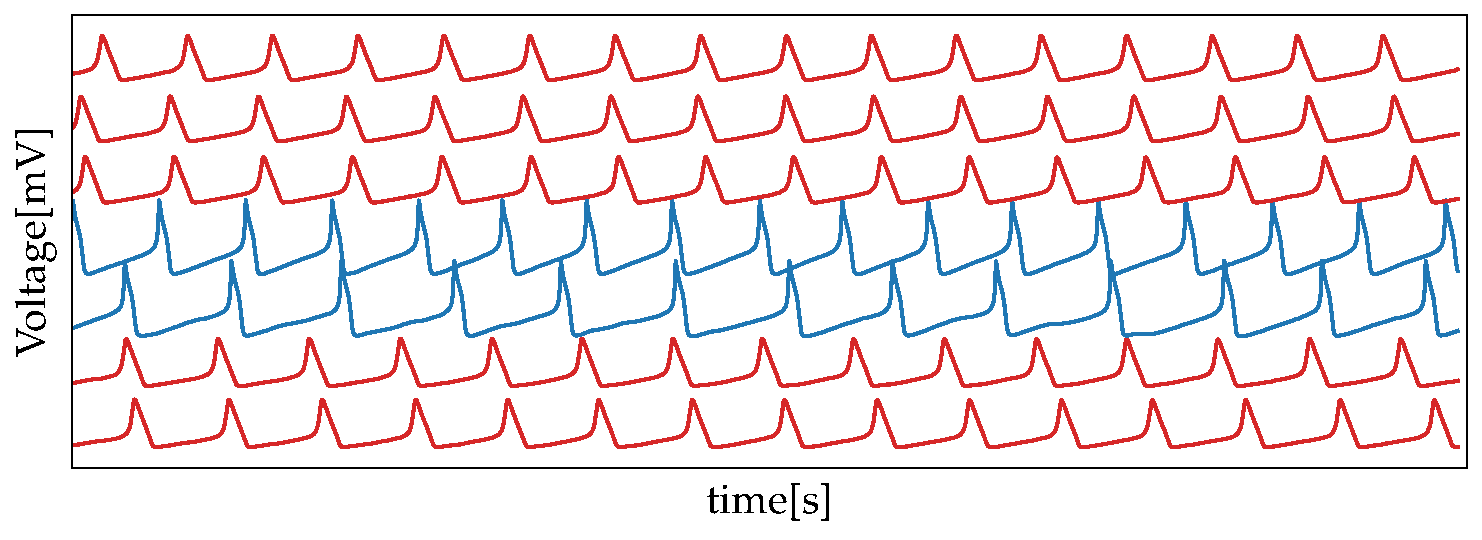
\includegraphics[width=0.9\columnwidth]{figs/snn_volt.pdf}
      \end{figure}
    \end{column}
    \begin{column}{0.5\textwidth}
      \checkmark 結合関数の推定
      \begin{figure}
        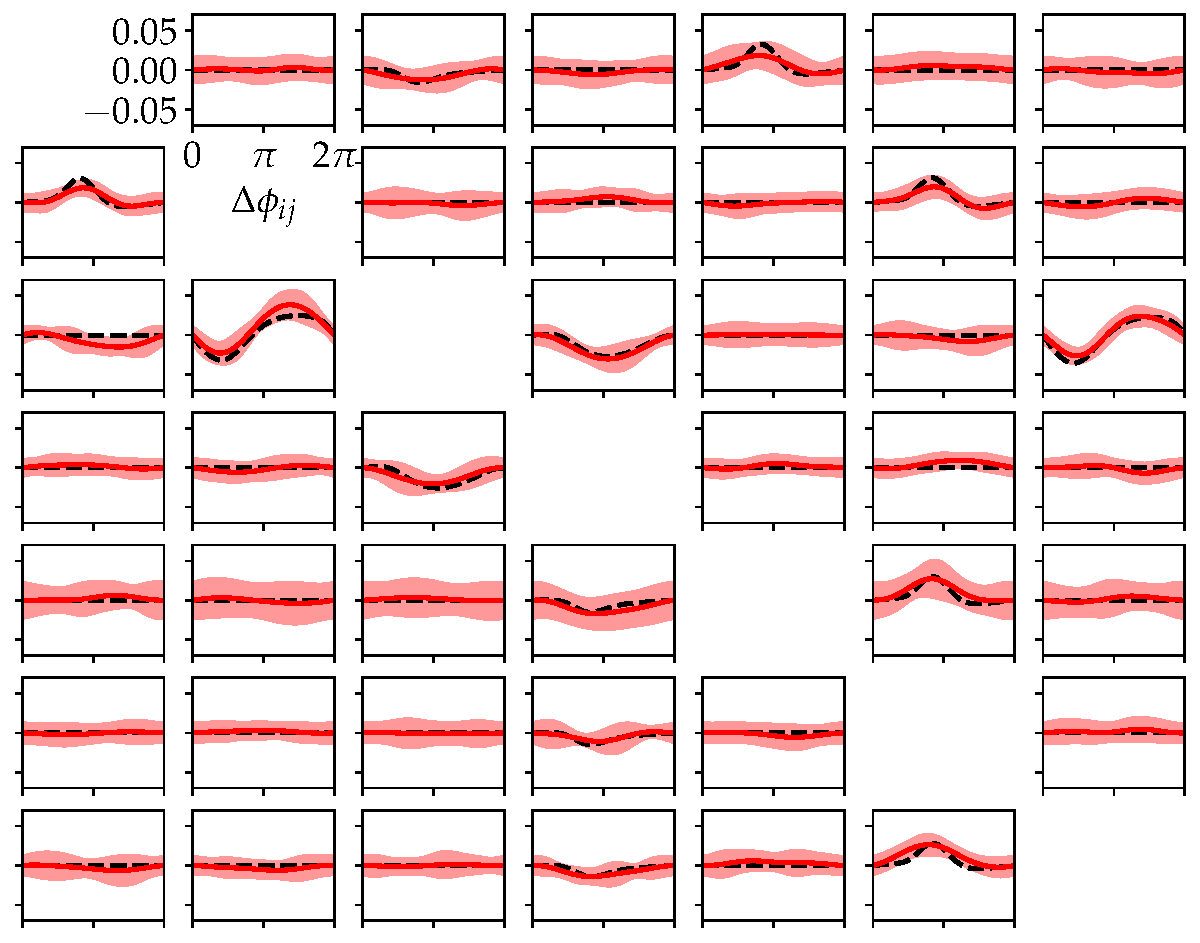
\includegraphics[width=\columnwidth]{figs/snn_gp_100.pdf}
        \caption*{黒点線: 理論\ \red{赤線: $\mathcal{GP}$回帰}}
      \end{figure}
    \end{column}
  \end{columns}
\end{frame}

\begin{frame}{まとめと展望}
  \begin{itemize}
    \item ガウス過程回帰を用いてリズム現象が従う結合位相振動子系を推定
    \begin{align*}
      k(\bm{x},\tilde{\bm{x}})=\sum_{j=1}^{N-1}p_{0}^{(j)}\exp(p_{1}^{(j)}\cos(x_{j}-\tilde{x}_{j}))
    \end{align*}
    \begin{figure}
      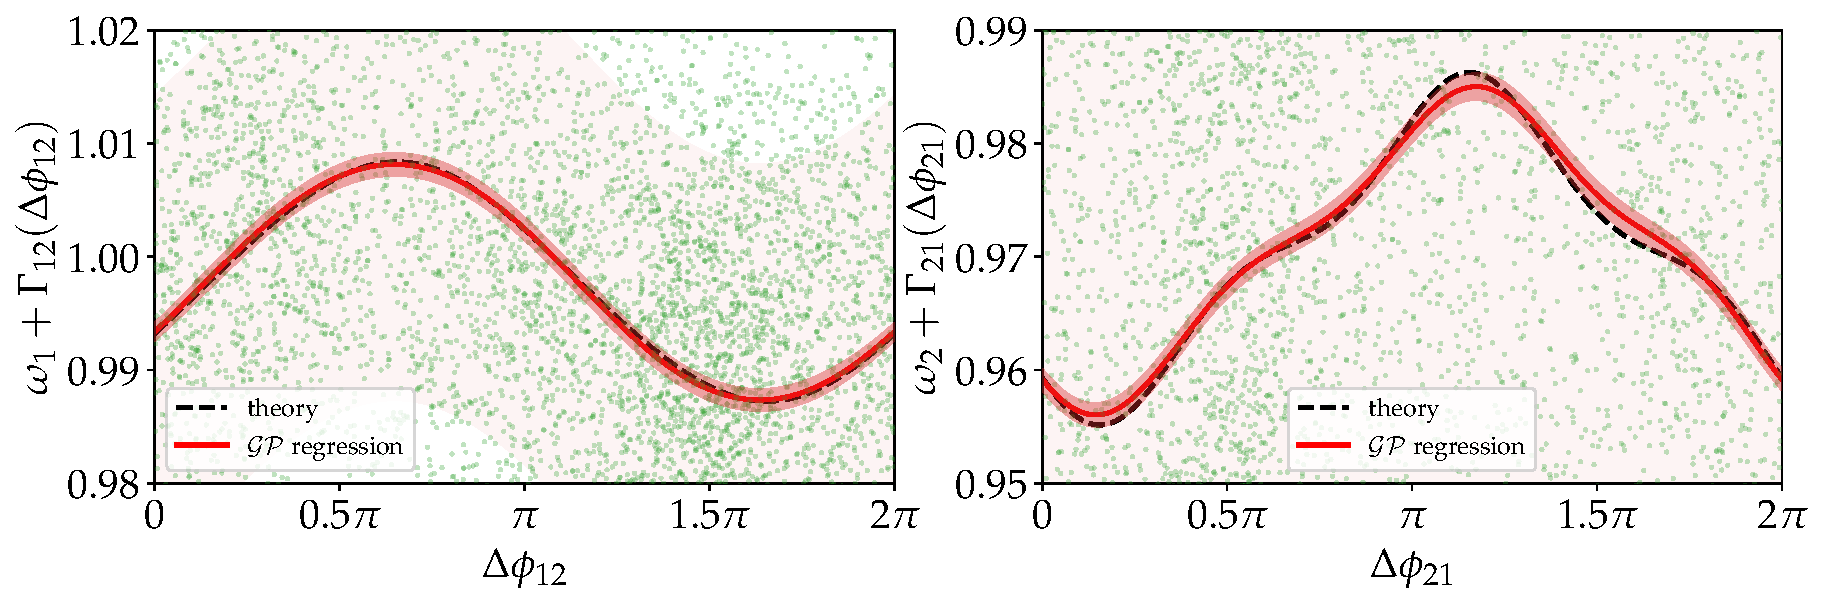
\includegraphics[height=0.3\textheight]{figs/exp01case01.pdf}
    \end{figure}
    \item 離散のデータから微分を近似するため誤差が生じる
    \begin{itemize}
      \item \textbf{Neural SDE} [Li 2020]によるベクトル場の回帰の検討 %\footnote{Ricky T. Q. Chen 2018}
      \begin{align*}
        \diff x=f(t,x;\theta_{f})\diff t+g(t,x;\theta_{g})\diff W_{t}
      \end{align*}
      \item 解軌道の$\theta_{f},\theta_{g}$微分をadjoint方程式で求める手法
    \end{itemize}
  \end{itemize}
\end{frame}